\documentclass[11pt]{article}
\usepackage[a4paper,margin=1in]{geometry}
\usepackage{amsmath,amssymb,amsthm,mathtools}
\usepackage{graphicx}
\usepackage{microtype}
\usepackage[hidelinks]{hyperref}

\newtheorem{theorem}{Theorem}
\newtheorem{lemma}{Lemma}
\newcommand{\E}{\mathbb E}
\newcommand{\R}{\mathbb R}
\newcommand{\N}{\mathbb N}
\newcommand{\sym}{\operatorname{sym}}
\newcommand{\epss}{\varepsilon_s}

\title{A Parity Classification for the Vanishing-Moment\\
Rademacher-Type Inequality}
\author{Automated Mathematics Run \texttt{fa\_banach\_001}, lane 2}
\date{9 August 2026}

\begin{document}
\maketitle

\begin{center}
\fbox{\parbox{0.91\textwidth}{\textbf{Status.}
Candidate full solution, likely valid.  The type-necessity question in
Remark 3.18 is answered completely: odd tensor orders characterize type,
whereas even orders are vacuous over the real scalar field.}}
\end{center}

\section{Source question}

Kirchner and Schwab~\cite{KS} prove in Corollary 3.17 that Rademacher type
$p$ implies their estimate (3.18) for independent random variables with
vanishing $k$th injective moment.  In Remark 3.18, pages 14--15, they ask
whether type $p$ is necessary.  The source statement spans the following two
page crops.

\begin{figure}[ht]
\centering
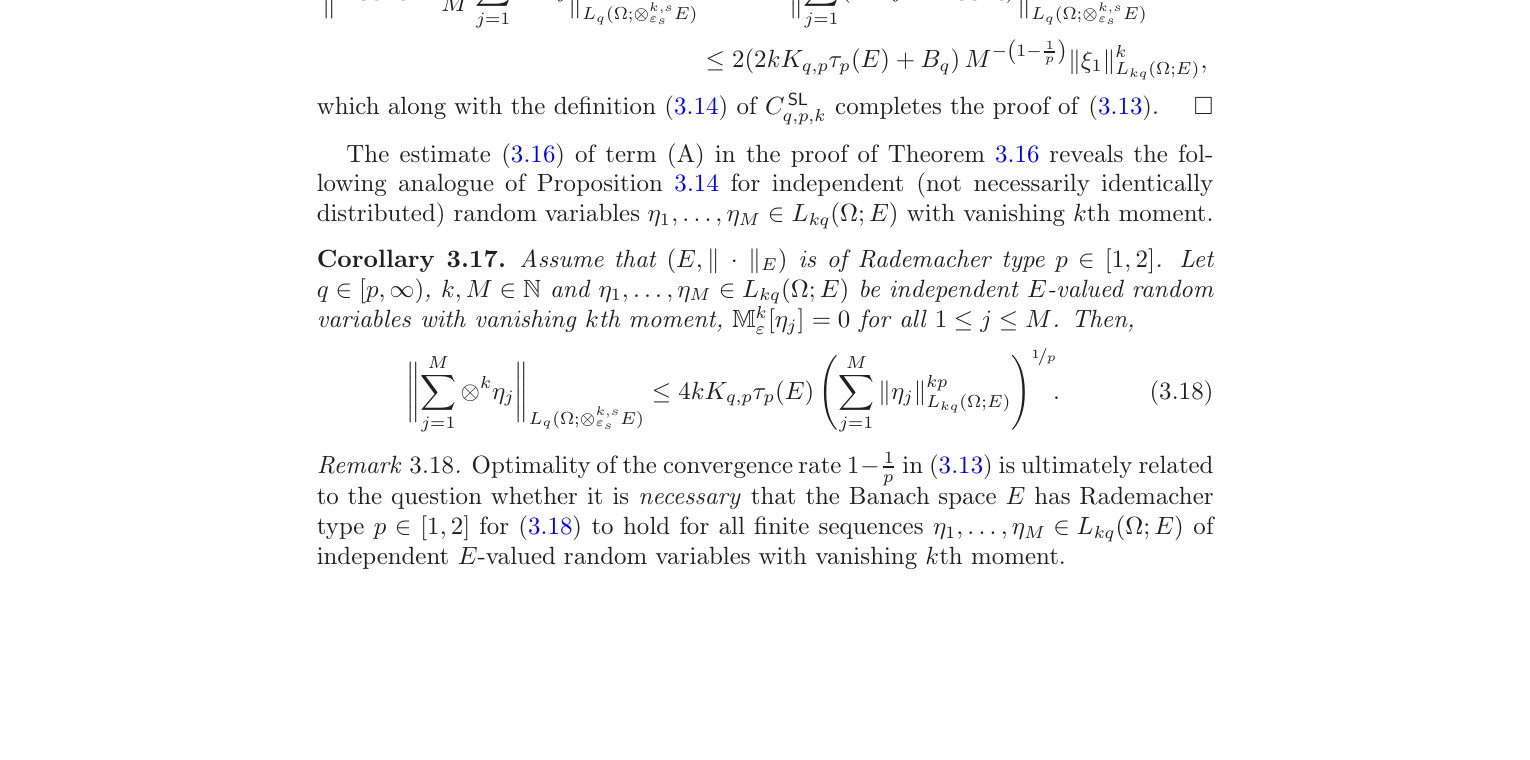
\includegraphics[width=\textwidth]{figures/open_problem_page14_crop.png}
\caption{Corollary 3.17 and the beginning of Remark 3.18 on source page 14.}
\end{figure}

\begin{figure}[ht]
\centering
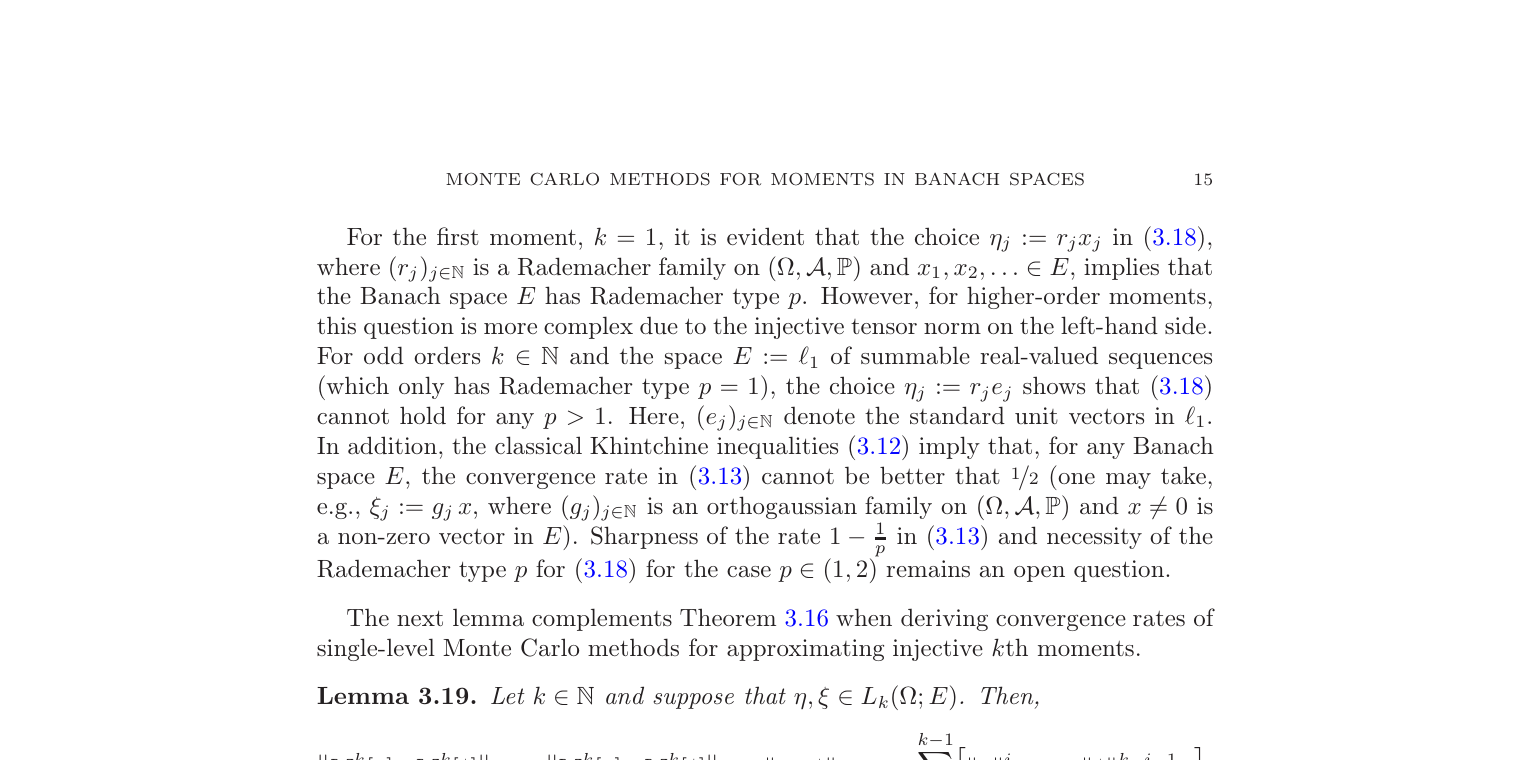
\includegraphics[width=\textwidth]{figures/open_problem_page15_crop.png}
\caption{The continuation and open-question sentence on source page 15.}
\end{figure}

For clarity, fix a real Banach space $E$, $1\le p\le2$, $q\ge p$, and
$k\ge2$.  Write $S^k_{\epss}E$ for the completed symmetric injective tensor
power, whose norm on a symmetric tensor $T$ is
\[
 \|T\|_{\epss}
 =\sup_{f\in B_{E^*}}|\langle T,f^{\otimes k}\rangle|.
\]
Let $\mathsf{VM}_{k,p,q}(E)$ denote the existence of a constant $C<\infty$
such that every finite independent family
$\eta_1,\ldots,\eta_M\in L_{kq}(\Omega;E)$ satisfying
$\E[\eta_j^{\otimes k}]=0$ obeys
\begin{equation}\label{eq:VM}
 \left\|\sum_{j=1}^M\eta_j^{\otimes k}\right\|_
 {L_q(\Omega;S^k_{\epss}E)}
 \le C\left(\sum_{j=1}^M
 \|\eta_j\|_{L_{kq}(\Omega;E)}^{kp}\right)^{1/p}.
\end{equation}

\section{Proof intuition}

Parity changes the question completely.  At even order, every repeated dual
evaluation of a zero tensor moment is the expectation of a nonnegative even
power.  Thus the random variable itself must vanish, so the estimate tests no
geometry at all.

At odd order, Rademacher signs turn any deterministic vector $z$ into an
admissible random variable $rz$.  Pure powers still hide the linear
Rademacher sum.  To recover it, split off a fixed transverse direction $y_0$
from a hyperplane $H$.  For $x\in H$, balance
$y=\|x\|^{1/k}y_0$ and
$u=\|x\|^{-(k-1)/k}x$.  Polynomial interpolation extracts the term linear in
$u$ from $(y+tu)^{\otimes k}$.  The balancing ensures that its $kp$-cost is
exactly $\|x\|^p$, while a functional equal to one on $y_0$ recovers the
ordinary Rademacher sum in $H$.

\section{Classification theorem}

\begin{theorem}[Parity classification]\label{thm:main}
Let $E$ be a real Banach space, $1\le p\le2$, $q\ge p$, and $k\ge2$.
\begin{enumerate}
\item If $k$ is odd, then $\mathsf{VM}_{k,p,q}(E)$ holds if and only if $E$
has Rademacher type $p$.
\item If $k$ is even, then every $E$-valued random variable with vanishing
$k$th injective moment is zero almost surely.  Consequently
$\mathsf{VM}_{k,p,q}(E)$ holds vacuously for every real Banach space $E$.
In particular, for every $p>1$, $E=\ell_1$ disproves necessity of type $p$.
\end{enumerate}
\end{theorem}

\subsection*{Even orders}

\begin{proof}[Proof of Theorem~\ref{thm:main}(2)]
Let $k$ be even and let $\eta\in L_{kq}(\Omega;E)$ satisfy
$\E[\eta^{\otimes k}]=0$.  Strong measurability gives a separable closed
subspace $E_0\subseteq E$ containing $\eta(\omega)$ almost surely.  There is a
sequence $(f_n)\subseteq B_{E^*}$ which norms $E_0$:
\[
 \|x\|=\sup_n|f_n(x)|,\qquad x\in E_0.
\]
Indeed, choose a dense sequence in the unit sphere of $E_0$, take norming
functionals there, and extend them to $E$ by Hahn--Banach.

Applying $f_n^{\otimes k}$ to the Bochner integral gives
\[
 0=\left\langle\E[\eta^{\otimes k}],f_n^{\otimes k}\right\rangle
  =\E[f_n(\eta)^k].
\]
The integrand is nonnegative because $k$ is even, so $f_n(\eta)=0$ almost
surely.  Intersecting the countably many full-measure events and using the
norming property gives $\eta=0$ almost surely.  Hence every family admissible
in \eqref{eq:VM} is identically zero.  The final assertion follows because
$\ell_1$ has no Rademacher type $p>1$.
\end{proof}

\subsection*{Odd orders: coefficient extraction}

For $0\le\ell\le k$, put
\begin{equation}\label{eq:coefficients}
 c_0=-\sum_{m=1}^k\frac1m,
 \qquad
 c_\ell=(-1)^{\ell-1}\frac1\ell\binom{k}{\ell}
 \quad(1\le\ell\le k).
\end{equation}
Lagrange interpolation at $0,1,\ldots,k$ implies that for every polynomial
$P$ of degree at most $k$, its coefficient of $t$ is
\begin{equation}\label{eq:extract}
 [t]P(t)=\sum_{\ell=0}^k c_\ell P(\ell).
\end{equation}
The formula follows by differentiating the Lagrange basis at zero.  In
particular, in the symmetric algebra over $E$,
\begin{equation}\label{eq:tensor-extract}
 k\,\sym(y^{\otimes(k-1)}\otimes u)
 =\sum_{\ell=0}^k c_\ell(y+\ell u)^{\otimes k}.
\end{equation}

\begin{proof}[Proof of Theorem~\ref{thm:main}(1)]
If $E$ has type $p$, property $\mathsf{VM}_{k,p,q}(E)$ is precisely the
sufficiency estimate proved in Corollary 3.17 of~\cite{KS}.  We prove the
converse.

Assume \eqref{eq:VM} with constant $C$ and let $k$ be odd.  Fix
$y_0\in S_E$ and $\psi\in S_{E^*}$ with $\psi(y_0)=1$.  Set
\[
 H=\ker\psi,
 \qquad P x=x-\psi(x)y_0.
\]
Then $P$ projects $E$ onto $H$ and $\|P\|\le2$.

Take arbitrary $x_1,\ldots,x_M\in H$.  If $x_j\ne0$, define
\[
 a_j=\|x_j\|^{1/k},\qquad
 y_j=a_jy_0,\qquad
 u_j=a_j^{-(k-1)}x_j;
\]
if $x_j=0$, set $a_j=y_j=u_j=0$.  Thus
\begin{equation}\label{eq:balanced}
 \|y_j+\ell u_j\|\le(1+\ell)a_j,
 \qquad a_j^{kp}=\|x_j\|^p.
\end{equation}

Let $r_1,\ldots,r_M$ be independent Rademacher signs.  For each fixed
$\ell$, the random variables
$\eta_{j,\ell}=r_j(y_j+\ell u_j)$ are independent and, since $k$ is odd,
\[
 \E[\eta_{j,\ell}^{\otimes k}]
 =\E[r_j^k](y_j+\ell u_j)^{\otimes k}=0.
\]
Applying \eqref{eq:VM} and \eqref{eq:balanced} gives
\begin{equation}\label{eq:pure-bound}
 \left\|\sum_jr_j(y_j+\ell u_j)^{\otimes k}\right\|_{L_q(S^k_{\epss}E)}
 \le C(1+\ell)^k
 \left(\sum_j\|x_j\|^p\right)^{1/p}.
\end{equation}

Put $T_j=\sym(y_j^{\otimes(k-1)}\otimes u_j)$ and
$D_k=\sum_{\ell=0}^k|c_\ell|(1+\ell)^k$.  Summing
\eqref{eq:tensor-extract} with signs and using \eqref{eq:pure-bound} yields
\begin{equation}\label{eq:mixed-upper}
 \left\|\sum_jr_jT_j\right\|_{L_q(S^k_{\epss}E)}
 \le \frac{CD_k}{k}
 \left(\sum_j\|x_j\|^p\right)^{1/p}.
\end{equation}

We now recover the ordinary Rademacher sum.  For each realization, let
$h=\sum_jr_jx_j\in H$ and choose $\phi\in B_{H^*}$ norming $h$ up to an
arbitrarily small error.  Define
\[
 f(x)=\phi(Px)+\psi(x),\qquad x\in E.
\]
Then $f(y_0)=1$, $f|_H=\phi$, and $\|f\|\le\|P\|+\|\psi\|\le3$.
Testing against $(f/3)^{\otimes k}$ and using the balanced definitions gives
\[
 \left\|\sum_jr_jT_j\right\|_{\epss}
 \ge 3^{-k}|\phi(h)|.
\]
Letting the norming error tend to zero, taking $L_q$-norms, and combining
with \eqref{eq:mixed-upper}, we obtain
\begin{equation}\label{eq:Htype}
 \left\|\sum_jr_jx_j\right\|_{L_q(E)}
 \le \frac{3^kCD_k}{k}
 \left(\sum_j\|x_j\|^p\right)^{1/p}.
\end{equation}
Since $q\ge p$, the same bound holds in $L_p$.  Thus $H$ has Rademacher
type $p$.

Finally, every $x\in E$ decomposes as $x=Px+\psi(x)y_0$.  For arbitrary
$x_1,\ldots,x_M\in E$, the triangle inequality, \eqref{eq:Htype}, and the
scalar Khintchine inequality give
\[
 \left\|\sum_jr_jx_j\right\|_{L_p(E)}
 \le 2\frac{3^kCD_k}{k}
       \left(\sum_j\|x_j\|^p\right)^{1/p}
    + \left(\sum_j|\psi(x_j)|^p\right)^{1/p}.
\]
Therefore $E$ has Rademacher type $p$.
\end{proof}

\section{Consequences, verification, and scope}

Theorem~\ref{thm:main} supplies a complete answer to the necessity question
for (3.18): affirmative at odd orders, negative and vacuous at even orders.
The source paper's separate question about sharpness of the i.i.d. Monte Carlo
rate (3.13) is not claimed here.

The exact script \texttt{code/verify\_interpolation.py} checked
\eqref{eq:extract} for every monomial of degree at most $k$ and all
$1\le k\le20$.  This check is not used as a substitute for the displayed
Lagrange proof.

A bounded literature search through 9 August 2026 covered the run indexes,
the current arXiv and published versions of~\cite{KS}, exact searches using
the phrases ``vanishing kth moment,'' ``Rademacher type,'' and ``injective
tensor,'' and the related follow-up arXiv:2605.24620.  No source recording the
parity classification or the balanced-polarization proof was found.  This is
not a novelty guarantee.

\paragraph{Human-review recommendation.}
Check the normalization in \eqref{eq:tensor-extract}, the balanced exponent in
\eqref{eq:balanced}, and the pointwise choice of the norming functional before
accepting the result as a full solution of the necessity question.

\begin{thebibliography}{9}
\bibitem{KS}
K.~Kirchner and C.~Schwab,
\emph{Monte Carlo convergence rates for kth moments in Banach spaces},
J. Funct. Anal. \textbf{286} (2024), Article 110218;
arXiv:2212.03797.
\end{thebibliography}

\end{document}

